\chapter{Methods}
\label{chap:methods}

As discussed in \autoref{chap:introduction}, the system developed in this thesis follows a pipeline consisting of two steps:
\begin{enumerate}
    \item \textbf{Object Proposal}: detection of all the logos in the image
    \item \textbf{Classification}: recognize each logo
\end{enumerate}
The first step regarding the detection of logos in the image is done by YOLO (see \autoref{sec:yolo}), while the actual recognition of the logo is performed by the classifier in an incremental learning setup. The pipeline of the system is shown in \autoref{fig:roi_and_classification}.

\begin{figure}%
	\centering

    \begin{center}
        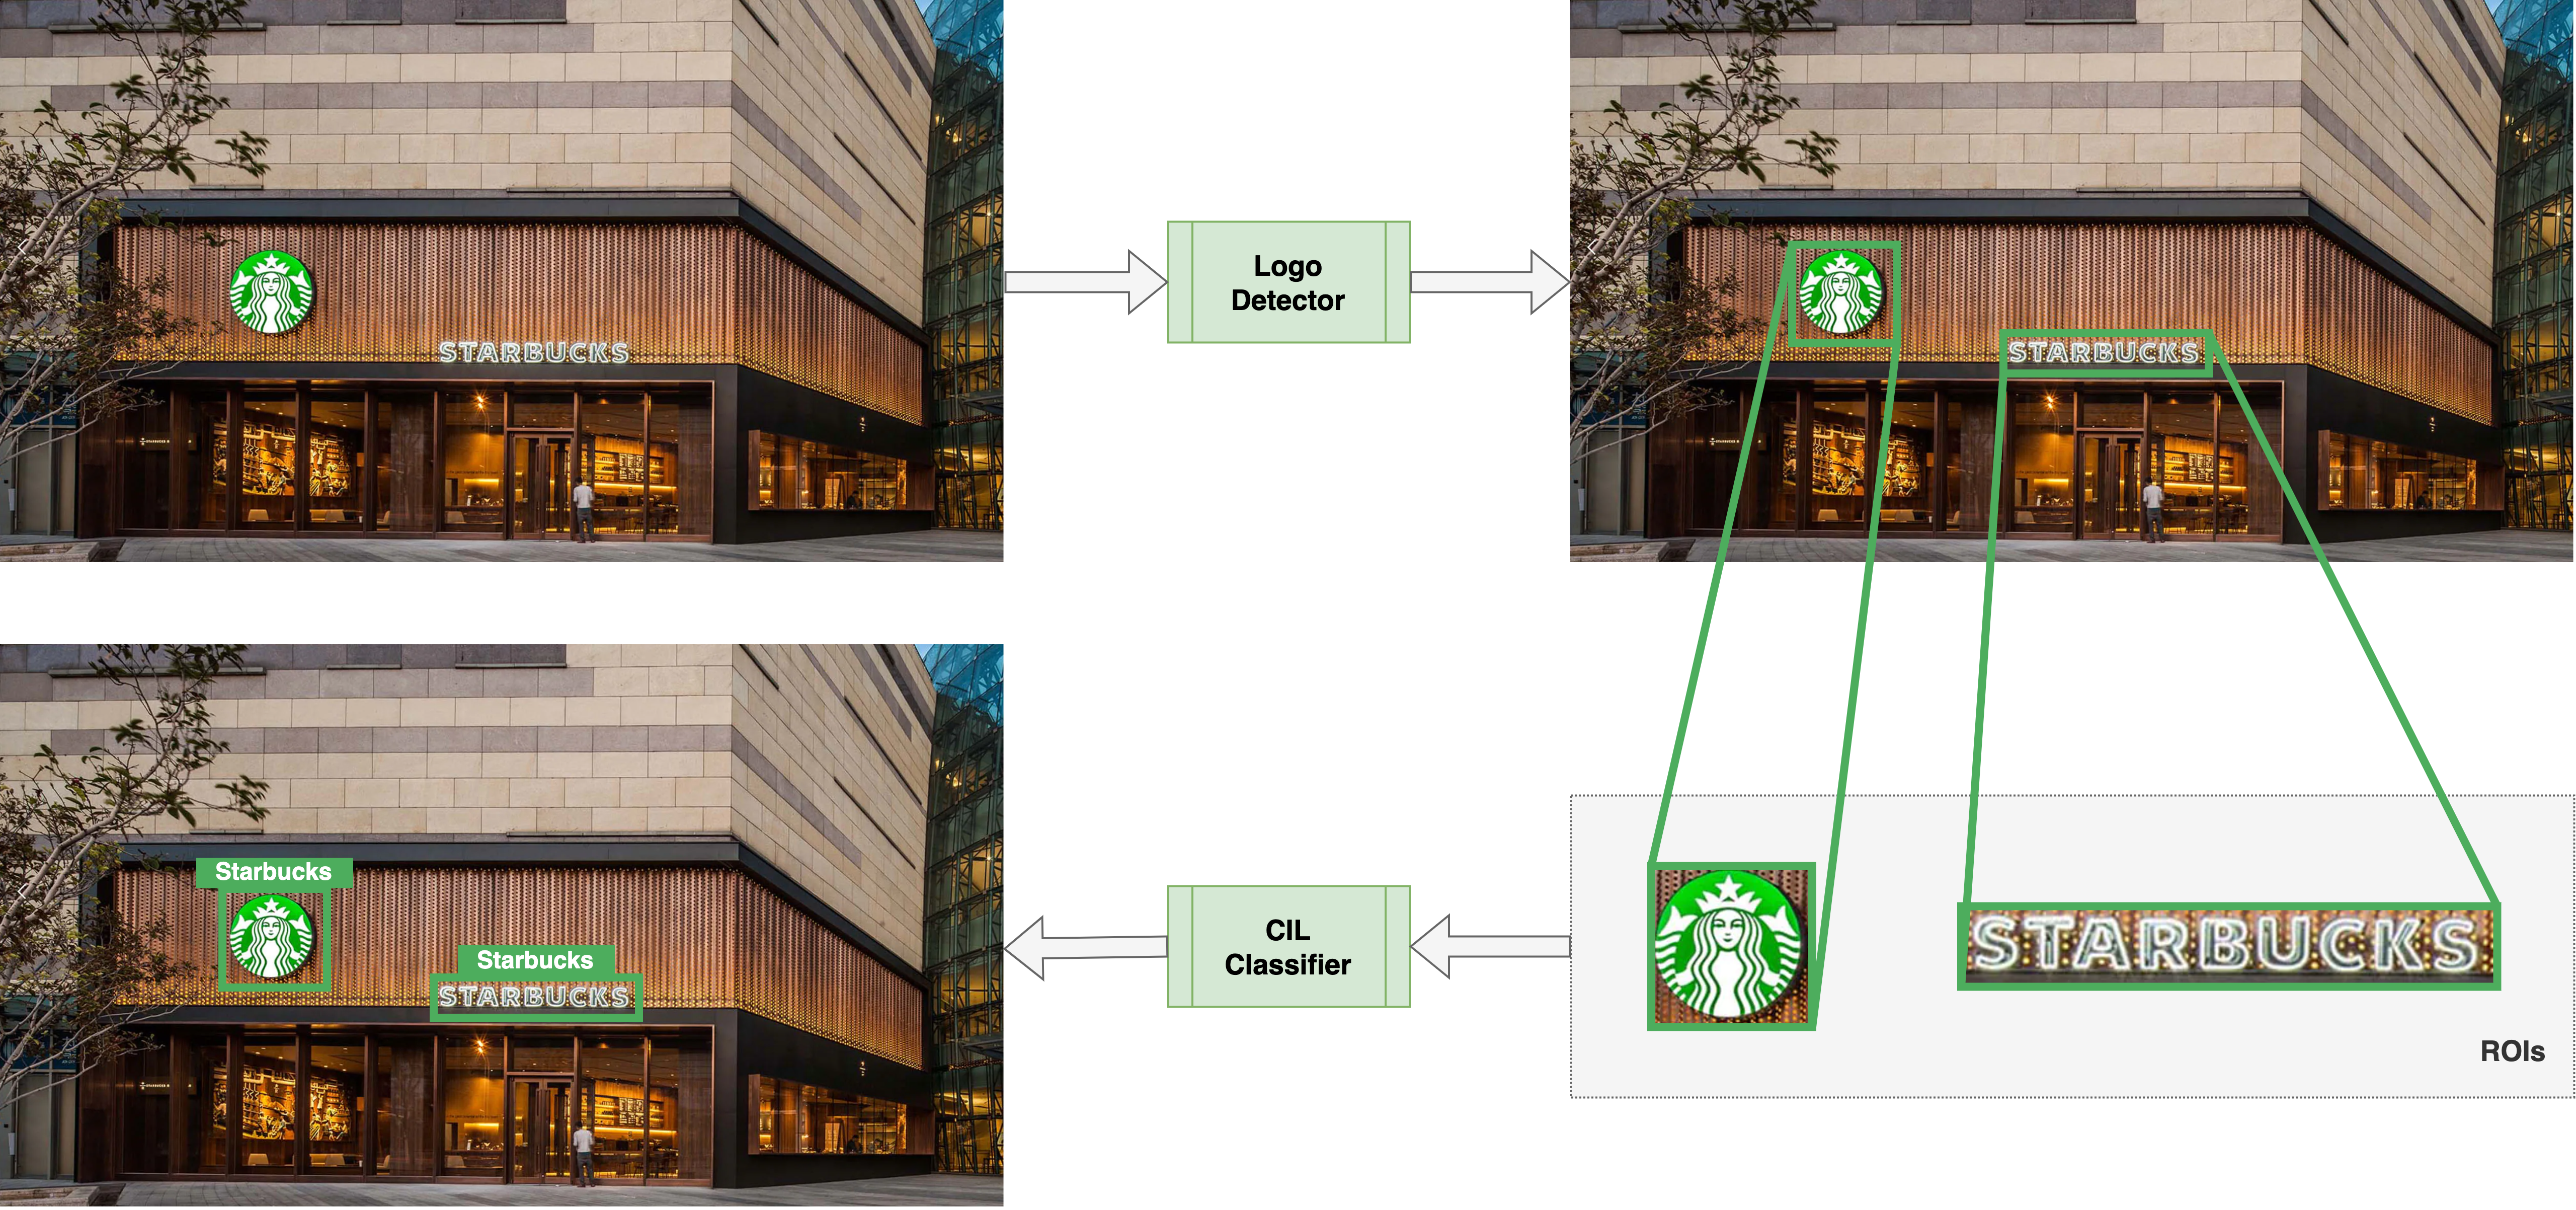
\includegraphics[width=\columnwidth]{images/roi+classification.drawio.png}
    \end{center}

	\caption{Pipeline of the system: the class-agnostic logo detector generates ROIs, then the classification is performed by the CIL classifier.}%
	\label{fig:roi_and_classification}%
\end{figure}

The detector used in the first step is a class-agnostic logo detector: it is a logo detector since we are not interested in the detection of objects other than logo; and it is class-agnostic since the number of detected classes is only one. In fact, in this first step the detector will be responsible for finding any generic logo (i.e., a single class) in the image. This is a crucial step if we seek to achieve incremental learning logo recognition, because in this way it is possible to decouple the detection from the recognition. If the logo detector localize any generic logo in the image, and delegates the actual recognition to the CIL classifier, there is no need to develop an incremental learning detector as well.

An important aspect of the classifier is the model size in terms of number of parameters. A big model comes with several disadvantages like longer time for the training phase, higher memory requirements and longer time to make inference. To this reason, a part of this work aims to decrease the number of parameters of the classifier using two different techniques. The first technique is described in \autoref{sec:method-pruning}, using masking and pruning described in \autoref{sec:masking-pruning} it aims to prune the model after the training of each incremental step, thus reducing the number of parameters. The second approach is the Knowledge Distillation (KD) described in \autoref{sec:method-kd}, where a smaller model is trained from scratch with the supervision of a bigger model trained on the same task.

This chapter describes all the details about the logo detector in \autoref{sec:method-roi} and continues with the classifier in \autoref{sec:method-classifier}. Then, in \autoref{sec:method-pruning} and \autoref{sec:method-kd} are discussed some techniques with the purpose to reducing the number of parameters of the model. In order to evaluate the drop in the terms of performance of the CIL classifier when compared to a standard close-set classification task (i.e. all the classes are available ath the beginning and there is no need to introduce new classes during time),
the chapter ends in \autoref{sec:method-baseline} with the introduction of different baselines.  


\section{Region proposal}
A key component of the system is the logo detector. Formally, this first step is an object detection task, where the objects we seek to detect are the logos in the image. The logo detector produces in output the coordinates of the bounding boxes corresponding to the logos in the image. The bounding boxes can be used to crop the portions of the images generating the regions of interest (ROIs). The ROIs corresponds to what the detector considers as any generic logo, and these can be directly used as input for the CIL model which classifies (i.e. recognize) the logo.


\label{sec:method-roi}
\subsection{YOLO}
The class-agnostic logo detector is based on YOLOv5m6 \cite{glenn_jocher_2021_5563715}.

Immagine delle diverse size di YOLO

Tabella delle diverse size di YOLO

\section{Classification}
Given the ROIs, the classification of each cropped region is performed by a model trained using CIL techniques. To achieve this goal, the classifier is trained using the DER algorithm \cite{yan2021dynamically} described in \autoref{sec:der-algorithm}.

The DER algorithm introduces a new feature extractor $\mathcal{F}_t$ at each incremental step. This feature extractor consists of a Convolutional Neural Network (CNN). In the developed system, the backbone of the CNN used as feature extractor is ResNet-34 \cite{he2016deep} pre-trained on ImageNet1000 \cite{deng2009imagenet}. The architecture of ResNet-34 is the following:


\begin{table}
    \centering
    \begingroup
    
    \begin{tabular}{>{\centering\arraybackslash}p{.3\textwidth}|>{\centering\arraybackslash}p{.3\textwidth}|>{\centering\arraybackslash}p{.3\textwidth}}
        \hline
        \textbf{Layer name} & \textbf{Output size} & \textbf{Layer} \\
        \hline
        \hline
        conv1 & $112 \times 122$ & $7 \times 7, 64,$ stride $2$ \\
        \hline
          & $56 \times 56$ & $3 \times 3$ max pool, stride $2$ \\
        \hline

        \[ \textrm{conv2\char`_x} \] &  \[56 \times 56 \] & \[\left[ \begin{array}{c} 3 \times 3, \, 64\\ 3 \times 3, \, 64  \end{array}\right] \times 3 \]\\
        \hline

        \[ \textrm{conv3\char`_x} \] &  \[28 \times 28 \] & \[\left[ \begin{array}{c} 3 \times 3, \, 128\\ 3 \times 3, \, 128  \end{array}\right] \times 4 \]\\
        \hline

        \[ \textrm{conv4\char`_x} \] &  \[14 \times 14 \] & \[\left[ \begin{array}{c} 3 \times 3, \, 256\\ 3 \times 3, \, 256  \end{array}\right] \times 6 \]\\
        \hline

        \[ \textrm{conv5\char`_x} \] &  \[7 \times 7 \] & \[\left[ \begin{array}{c} 3 \times 3, \, 512\\ 3 \times 3, \, 512  \end{array}\right] \times 3 \]\\
        \hline
        & $1000 \times 1$ & average pool \\
        \hline
        FC & $1000 \times 1$ & $1000$-d FC layer, softmax \\
        \hline
        \end{tabular}
    \endgroup
    \caption{Ciao}
\end{table}

\end{document}

\label{sec:method-classifier}
\subsection{Regularization techniques}
\subsection{Data Augmentation}
\subsection{Pruning}
\label{sec:method-pruning}
\section{Knowledge distillation}

\label{sec:method-kd}
\section{Proposed baseline for the classifier}
\label{sec:method-baseline}
\subsection{Baseline without incremental steps}
\subsection{ResNet-152 architecture}
\subsection{DER-based architecture}